
Nguyên lý Scheimpflug được đặt theo tên của kỹ sư người Áo Theodor Scheimpflug, mô tả cách một mặt phẳng tiêu cự có thể nghiêng để mở rộng vùng ảnh rõ nét trong nhiếp ảnh và quang học. 

Cụ thể, nguyên lý Scheimpflug phát biểu rằng khi mặt phẳng vật, mặt phẳng thấu kính và mặt phẳng ảnh (cảm biến hoặc phim) không song song mà giao nhau tại một đường thẳng chung, thì toàn bộ mặt phẳng vật nghiêng này vẫn có thể được lấy nét rõ ràng. 
\begin{enumerate}[label=(\alph*)]
\item Chứng minh nguyên lý Scheimpflug
\item Chứng minh rằng mặt phẳng tiêu cự quay quanh một trục đi qua điểm G khi ta nghiêng thấu kính \\
\begin{figure}[H]
    \centering
    \tikzset{every picture/.style={line width=0.75pt}} %set default line width to 0.75pt        

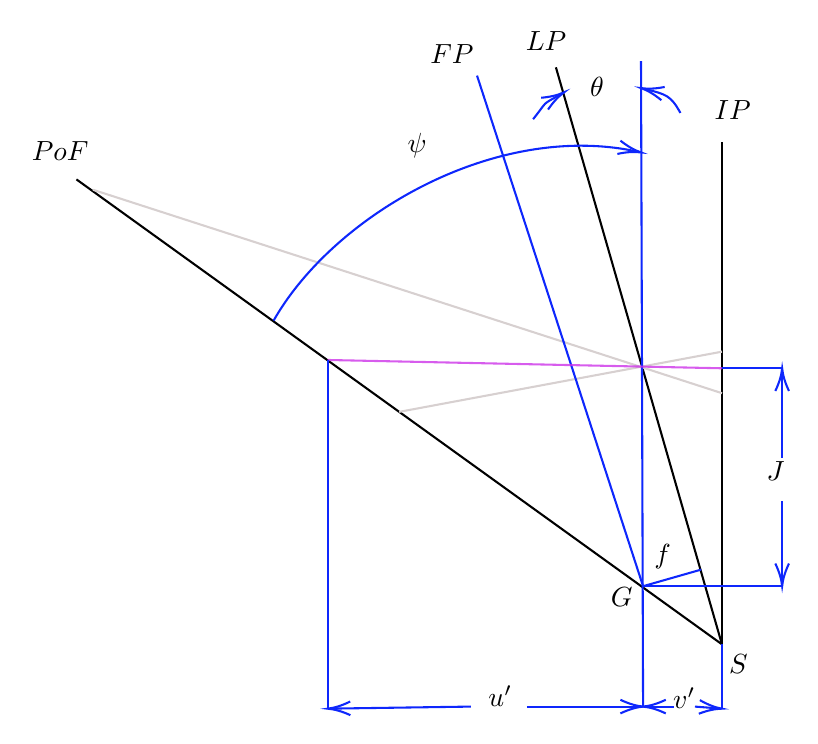
\begin{tikzpicture}[x=0.75pt,y=0.75pt,yscale=-1,xscale=1]
%uncomment if require: \path (0,424); %set diagram left start at 0, and has height of 424

%Straight Lines [id:da17793481393532118] 
\draw    (100,106) -- (411,330) ;
%Straight Lines [id:da4232639599589497] 
\draw    (411,88) -- (411,330) ;
%Straight Lines [id:da11938100176501354] 
\draw    (331,52) -- (411,330) ;
%Straight Lines [id:da838504233570497] 
\draw [color={rgb, 255:red, 215; green, 208; blue, 208 }  ,draw opacity=1 ]   (108,111) -- (411,209) ;
%Straight Lines [id:da49314275647124217] 
\draw [color={rgb, 255:red, 215; green, 208; blue, 208 }  ,draw opacity=1 ]   (255.5,218) -- (411,189) ;
%Straight Lines [id:da48246879037954804] 
\draw [color={rgb, 255:red, 14; green, 39; blue, 252 }  ,draw opacity=1 ]   (372,49) -- (373,360) ;
%Curve Lines [id:da20103497237081303] 
\draw [color={rgb, 255:red, 14; green, 39; blue, 252 }  ,draw opacity=1 ]   (195,174) .. controls (223.86,123.25) and (302.21,77.46) .. (370.96,92.76) ;
\draw [shift={(372,93)}, rotate = 193.06] [color={rgb, 255:red, 14; green, 39; blue, 252 }  ,draw opacity=1 ][line width=0.75]    (10.93,-3.29) .. controls (6.95,-1.4) and (3.31,-0.3) .. (0,0) .. controls (3.31,0.3) and (6.95,1.4) .. (10.93,3.29)   ;
%Curve Lines [id:da766499281537382] 
\draw [color={rgb, 255:red, 14; green, 39; blue, 252 }  ,draw opacity=1 ]   (320,77) .. controls (327.6,67.5) and (323.47,70.64) .. (333.32,64.97) ;
\draw [shift={(335,64)}, rotate = 149.74] [color={rgb, 255:red, 14; green, 39; blue, 252 }  ,draw opacity=1 ][line width=0.75]    (10.93,-3.29) .. controls (6.95,-1.4) and (3.31,-0.3) .. (0,0) .. controls (3.31,0.3) and (6.95,1.4) .. (10.93,3.29)   ;
%Curve Lines [id:da17003487311025278] 
\draw [color={rgb, 255:red, 14; green, 39; blue, 252 }  ,draw opacity=1 ]   (391,74) .. controls (386.28,65.49) and (384.23,65.03) .. (373.89,62.47) ;
\draw [shift={(372,62)}, rotate = 14.04] [color={rgb, 255:red, 14; green, 39; blue, 252 }  ,draw opacity=1 ][line width=0.75]    (10.93,-3.29) .. controls (6.95,-1.4) and (3.31,-0.3) .. (0,0) .. controls (3.31,0.3) and (6.95,1.4) .. (10.93,3.29)   ;
%Straight Lines [id:da9027721988306059] 
\draw [color={rgb, 255:red, 14; green, 39; blue, 252 }  ,draw opacity=1 ][fill={rgb, 255:red, 14; green, 39; blue, 252 }  ,fill opacity=1 ]   (293,56) -- (373,302) ;
%Straight Lines [id:da5757635442365009] 
\draw [color={rgb, 255:red, 204; green, 48; blue, 232 }  ,draw opacity=0.79 ]   (221,193) -- (411,197) ;
%Straight Lines [id:da515546325781679] 
\draw [color={rgb, 255:red, 14; green, 39; blue, 252 }  ,draw opacity=1 ]   (373,302) -- (401,294) ;
%Straight Lines [id:da07987517143448997] 
\draw [color={rgb, 255:red, 14; green, 39; blue, 252 }  ,draw opacity=1 ]   (411,197) -- (440,197) ;
%Straight Lines [id:da32954315898274145] 
\draw [color={rgb, 255:red, 14; green, 39; blue, 252 }  ,draw opacity=1 ]   (373,302) -- (440,302) ;
%Straight Lines [id:da7673507644962323] 
\draw [color={rgb, 255:red, 14; green, 39; blue, 252 }  ,draw opacity=1 ]   (440,240) -- (440,199) ;
\draw [shift={(440,197)}, rotate = 90] [color={rgb, 255:red, 14; green, 39; blue, 252 }  ,draw opacity=1 ][line width=0.75]    (10.93,-3.29) .. controls (6.95,-1.4) and (3.31,-0.3) .. (0,0) .. controls (3.31,0.3) and (6.95,1.4) .. (10.93,3.29)   ;
%Straight Lines [id:da3847843275842151] 
\draw [color={rgb, 255:red, 14; green, 39; blue, 252 }  ,draw opacity=1 ]   (440,261) -- (440,300) ;
\draw [shift={(440,302)}, rotate = 270] [color={rgb, 255:red, 14; green, 39; blue, 252 }  ,draw opacity=1 ][line width=0.75]    (10.93,-3.29) .. controls (6.95,-1.4) and (3.31,-0.3) .. (0,0) .. controls (3.31,0.3) and (6.95,1.4) .. (10.93,3.29)   ;
%Straight Lines [id:da20281608213079083] 
\draw [color={rgb, 255:red, 14; green, 39; blue, 252 }  ,draw opacity=1 ]   (221,193) -- (221,361) ;
%Straight Lines [id:da1408913001205767] 
\draw [color={rgb, 255:red, 14; green, 39; blue, 252 }  ,draw opacity=1 ]   (411,330) -- (411,361) ;
%Straight Lines [id:da8412446681679657] 
\draw [color={rgb, 255:red, 14; green, 39; blue, 252 }  ,draw opacity=1 ]   (290,360) -- (223,360.97) ;
\draw [shift={(221,361)}, rotate = 359.17] [color={rgb, 255:red, 14; green, 39; blue, 252 }  ,draw opacity=1 ][line width=0.75]    (10.93,-3.29) .. controls (6.95,-1.4) and (3.31,-0.3) .. (0,0) .. controls (3.31,0.3) and (6.95,1.4) .. (10.93,3.29)   ;
%Straight Lines [id:da9709846088927524] 
\draw [color={rgb, 255:red, 14; green, 39; blue, 252 }  ,draw opacity=1 ]   (317,360) -- (371,360) ;
\draw [shift={(373,360)}, rotate = 180] [color={rgb, 255:red, 14; green, 39; blue, 252 }  ,draw opacity=1 ][line width=0.75]    (10.93,-3.29) .. controls (6.95,-1.4) and (3.31,-0.3) .. (0,0) .. controls (3.31,0.3) and (6.95,1.4) .. (10.93,3.29)   ;
%Straight Lines [id:da3803562259739416] 
\draw [color={rgb, 255:red, 14; green, 39; blue, 252 }  ,draw opacity=1 ]   (398,360) -- (409.01,360.85) ;
\draw [shift={(411,361)}, rotate = 184.4] [color={rgb, 255:red, 14; green, 39; blue, 252 }  ,draw opacity=1 ][line width=0.75]    (10.93,-3.29) .. controls (6.95,-1.4) and (3.31,-0.3) .. (0,0) .. controls (3.31,0.3) and (6.95,1.4) .. (10.93,3.29)   ;
%Straight Lines [id:da20928323034235796] 
\draw [color={rgb, 255:red, 14; green, 39; blue, 252 }  ,draw opacity=1 ]   (388,360) -- (375,360) ;
\draw [shift={(373,360)}, rotate = 360] [color={rgb, 255:red, 14; green, 39; blue, 252 }  ,draw opacity=1 ][line width=0.75]    (10.93,-3.29) .. controls (6.95,-1.4) and (3.31,-0.3) .. (0,0) .. controls (3.31,0.3) and (6.95,1.4) .. (10.93,3.29)   ;

% Text Node
\draw (346,55.4) node [anchor=north west][inner sep=0.75pt]    {$\theta $};
% Text Node
\draw (258,82.4) node [anchor=north west][inner sep=0.75pt]    {$\psi $};
% Text Node
\draw (356,301.4) node [anchor=north west][inner sep=0.75pt]    {$\text{G}$};
% Text Node
\draw (77,86.4) node [anchor=north west][inner sep=0.75pt]    {$\text{PoF}$};
% Text Node
\draw (269,39.4) node [anchor=north west][inner sep=0.75pt]    {$\text{FP}$};
% Text Node
\draw (315,33.4) node [anchor=north west][inner sep=0.75pt]    {$\text{LP}$};
% Text Node
\draw (406,66.4) node [anchor=north west][inner sep=0.75pt]    {$\text{IP}$};
% Text Node
\draw (413,333.4) node [anchor=north west][inner sep=0.75pt]    {$\text{S}$};
% Text Node
\draw (377,280.4) node [anchor=north west][inner sep=0.75pt]    {$\text{f}$};
% Text Node
\draw (431,240.4) node [anchor=north west][inner sep=0.75pt]    {$\text{J}$};
% Text Node
\draw (297,348.4) node [anchor=north west][inner sep=0.75pt]    {$\text{u'}$};
% Text Node
\draw (386,349.4) node [anchor=north west][inner sep=0.75pt]    {$\text{v'}$};
\end{tikzpicture}
\centering
\caption{}
    \label{fig:P2_01}
\end{figure}
\begin{enumerate}[label={}]
    \item IP=mặt phẳng ảnh
    \item LP=mặt phẳng thấu kính
    \item FP=mặt phẳng tiêu điểm trước (mặt phẳng song song LP và đi qua F)
    \item PoF=mặt phẳng tiêu cự
\end{enumerate}
\end{enumerate}
Một nghiên cứu sử dụng nguyên lý Scheimpflug và hệ thấu kính nghiêng để mô hình hóa hình dạng 3D của đồ vật. Bằng cách đặt vật thể trên một bệ dịch chuyển và cho chuyển động thẳng với tốc độ đồng đều rồi chụp ở mọi khoảng cách đã định, ta sẽ ghi lại được đường nét của vật. Bố trí thí nghiệm của nghiên cứu được cho ở hình vẽ bên dưới: 
\begin{figure}[H]
    \centering
   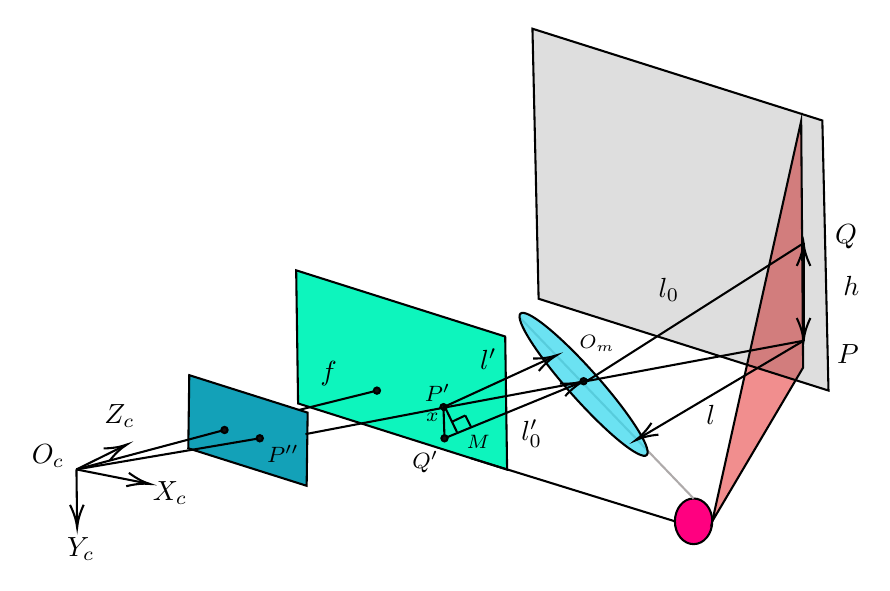
\begin{tikzpicture}[x=0.75pt,y=0.75pt,yscale=-1,xscale=1]
% Uncomment if required: \path (0,424); % set diagram left start at 0, and has height of 424

% Shape: Parallelogram [id:dp00958650764397817] 
\draw [fill={rgb, 255:red, 19; green, 161; blue, 184}, fill opacity=1] 
  (181.39,232.64) -- (124.36,214.59) -- (123.88,249.83) -- (180.91,267.88) -- cycle ;

% Shape: Parallelogram [id:dp022474278506247614] 
\draw [fill={rgb, 255:red, 13; green, 245; blue, 189}, fill opacity=1] 
  (276.57,195.97) -- (175.86,164.08) -- (176.78,228.21) -- (277.49,260.1) -- cycle ;

% Straight Lines [id:da8907782196447741]
\draw (260.02,254.57) -- (358.33,285) ;

% Shape: Ellipse [id:dp05488901106901134]
\draw [fill={rgb, 255:red, 255; green, 0; blue, 128}, fill opacity=1] 
  (358.33,285)
  .. controls (358.33,278.92) and (362.36,274) .. (367.33,274)
  .. controls (372.3,274) and (376.33,278.92) .. (376.33,285)
  .. controls (376.33,291.08) and (372.3,296) .. (367.33,296)
  .. controls (362.36,296) and (358.33,291.08) .. (358.33,285) -- cycle ;

% Straight Lines [id:da7460212634378354]
\draw [color={rgb, 255:red, 174; green, 170; blue, 170}, draw opacity=1]
  (283.47,186.65) -- (367.33,274) ;

% Shape: Triangle [id:dp18484560531905792]
\draw [fill={rgb, 255:red, 225; green, 18; blue, 18}, fill opacity=0.48]
  (419.17,92.13) -- (376.33,285) -- (420.11,210.91) -- cycle ;

% Shape: Parallelogram [id:dp2907384191063157]
\draw [fill={rgb, 255:red, 23; green, 23; blue, 23}, fill opacity=0.14]
  (429.37,91.89) -- (289.7,47.67) -- (292.67,177.78) -- (432.33,222) -- cycle ;

% Shape: Ellipse [id:dp3004682236426569]
\draw [fill={rgb, 255:red, 58; green, 216; blue, 237}, fill opacity=0.75]
  (313.45,207.21)
  .. controls (330.49,225.08) and (344.71,244.84) .. (345.19,251.35)
  .. controls (345.68,257.86) and (332.26,248.65) .. (315.22,230.79)
  .. controls (298.17,212.92) and (283.96,193.16) .. (283.47,186.65)
  .. controls (282.99,180.14) and (296.41,189.35) .. (313.45,207.21) -- cycle ;

% Straight Lines with Arrowheads
\draw (70,260) -- (92.54,248.88);
\draw [shift={(94.33,248)}, rotate=153.75, color=black, line width=0.75]
  (10.93,-3.29) .. controls (6.95,-1.4) and (3.31,-0.3) .. (0,0) 
  .. controls (3.31,0.3) and (6.95,1.4) .. (10.93,3.29);

\draw (70,260) -- (103.37,266.61);
\draw [shift={(105.33,267)}, rotate=191.21, color=black, line width=0.75]
  (10.93,-3.29) .. controls (6.95,-1.4) and (3.31,-0.3) .. (0,0) 
  .. controls (3.31,0.3) and (6.95,1.4) .. (10.93,3.29);

\draw (70,260) -- (70.31,286);
\draw [shift={(70.33,288)}, rotate=269.32, color=black, line width=0.75]
  (10.93,-3.29) .. controls (6.95,-1.4) and (3.31,-0.3) .. (0,0) 
  .. controls (3.31,0.3) and (6.95,1.4) .. (10.93,3.29);

\draw (70,260) -- (158.33,245);
\draw (180.33,243) -- (248.33,230);
\draw (70,260) -- (141.33,241);
\draw (177.44,231.29) -- (214.76,222.04);

% Shape: Circle
\draw [fill={rgb, 255:red, 18; green, 16; blue, 16}, fill opacity=1]
  (139.83,241)
  .. controls (139.83,240.17) and (140.5,239.5) .. (141.33,239.5)
  .. controls (142.16,239.5) and (142.83,240.17) .. (142.83,241)
  .. controls (142.83,241.83) and (142.16,242.5) .. (141.33,242.5)
  .. controls (140.5,242.5) and (139.83,241.83) .. (139.83,241) -- cycle ;

\draw [fill={rgb, 255:red, 18; green, 16; blue, 16}, fill opacity=1]
  (156.83,245)
  .. controls (156.83,244.17) and (157.5,243.5) .. (158.33,243.5)
  .. controls (159.16,243.5) and (159.83,244.17) .. (159.83,245)
  .. controls (159.83,245.83) and (159.16,246.5) .. (158.33,246.5)
  .. controls (157.5,246.5) and (156.83,245.83) .. (156.83,245) -- cycle ;

\draw [fill={rgb, 255:red, 18; green, 16; blue, 16}, fill opacity=1]
  (213.26,222.04)
  .. controls (213.26,221.21) and (213.94,220.54) .. (214.76,220.54)
  .. controls (215.59,220.54) and (216.26,221.21) .. (216.26,222.04)
  .. controls (216.26,222.87) and (215.59,223.54) .. (214.76,223.54)
  .. controls (213.94,223.54) and (213.26,222.87) .. (213.26,222.04) -- cycle ;

\draw [fill={rgb, 255:red, 18; green, 16; blue, 16}, fill opacity=1]
  (245.33,230)
  .. controls (245.33,229.17) and (246,228.5) .. (246.83,228.5)
  .. controls (247.66,228.5) and (248.33,229.17) .. (248.33,230)
  .. controls (248.33,230.83) and (247.66,231.5) .. (246.83,231.5) -- cycle ;

\draw (420.33,198) -- (248.33,230);

\draw [fill={rgb, 255:red, 18; green, 16; blue, 16}, fill opacity=1]
  (312.83,217.5)
  .. controls (312.83,216.67) and (313.5,216) .. (314.33,216)
  .. controls (315.16,216) and (315.83,216.67) .. (315.83,217.5)
  .. controls (315.83,218.33) and (315.16,219) .. (314.33,219)
  .. controls (313.5,219) and (312.83,218.33) .. (312.83,217.5) -- cycle ;

\draw (315.83,217.5) -- (420.33,151);
\draw (420.33,198) -- (341.05,244.98);
\draw [shift={(339.33,246)}, rotate=329.35, color=black, line width=0.75]
  (10.93,-3.29) .. controls (6.95,-1.4) and (3.31,-0.3) .. (0,0) 
  .. controls (3.31,0.3) and (6.95,1.4) .. (10.93,3.29);

\draw (246.83,230) -- (299.52,205.83);
\draw [shift={(301.33,205)}, rotate=155.36, color=black, line width=0.75]
  (10.93,-3.29) .. controls (6.95,-1.4) and (3.31,-0.3) .. (0,0)
  .. controls (3.31,0.3) and (6.95,1.4) .. (10.93,3.29);

\draw (246.83,230) -- (247.33,245);
\draw (247.33,245) -- (312.48,218.26);
\draw [shift={(314.33,217.5)}, rotate=157.68, color=black, line width=0.75]
  (10.93,-3.29) .. controls (6.95,-1.4) and (3.31,-0.3) .. (0,0)
  .. controls (3.31,0.3) and (6.95,1.4) .. (10.93,3.29);

\draw (420.33,198) -- (420.33,153);
\draw [shift={(420.33,151)}, rotate=90, color=black, line width=0.75]
  (10.93,-3.29) .. controls (6.95,-1.4) and (3.31,-0.3) .. (0,0)
  .. controls (3.31,0.3) and (6.95,1.4) .. (10.93,3.29);

\draw (420.33,151) -- (420.33,196);
\draw [shift={(420.33,198)}, rotate=270, color=black, line width=0.75]
  (10.93,-3.29) .. controls (6.95,-1.4) and (3.31,-0.3) .. (0,0)
  .. controls (3.31,0.3) and (6.95,1.4) .. (10.93,3.29);

\draw [fill={rgb, 255:red, 18; green, 16; blue, 16}, fill opacity=1]
  (245.83,245)
  .. controls (245.83,244.17) and (246.5,243.5) .. (247.33,243.5)
  .. controls (248.16,243.5) and (248.83,244.17) .. (248.83,245)
  .. controls (248.83,245.83) and (248.16,246.5) .. (247.33,246.5)
  .. controls (246.5,246.5) and (245.83,245.83) .. (245.83,245) -- cycle ;

\draw (246.83,228.5) -- (253.33,242);
\draw (251,237) -- (257.33,234);
\draw (257.33,234) -- (260.33,240);

% Text Nodes
\draw (47,246.4) node [anchor=north west, inner sep=0.75pt] {$\text{O}_{c}$};
\draw (82,227.4) node [anchor=north west, inner sep=0.75pt] {$\text{Z}_{c}$};
\draw (105.33,264.4) node [anchor=north west, inner sep=0.75pt] {$\text{X}_{c}$};
\draw (64,291.4) node [anchor=north west, inner sep=0.75pt] {$\text{Y}_{c}$};
\draw (186,206.4) node [anchor=north west, inner sep=0.75pt] {$\text{f}$};
\draw (236.33,217.4) node [anchor=north west, inner sep=0.75pt, font=\footnotesize] {$\text{P}'$};
\draw (263,200.4) node [anchor=north west, inner sep=0.75pt] {$\text{l}'$};
\draw (438,165.4) node [anchor=north west, inner sep=0.75pt] {$\text{h}$};
\draw (282.83,234.65) node [anchor=north west, inner sep=0.75pt] {$\text{l}'_{0}$};
\draw (310.83,193.9) node [anchor=north west, inner sep=0.75pt, font=\scriptsize] {$\text{O}_{m}$};
\draw (237,231.4) node [anchor=north west, inner sep=0.75pt, font=\scriptsize] {$\text{x}$};
\draw (230.33,249.9) node [anchor=north west, inner sep=0.75pt, font=\footnotesize] {$\text{Q}'$};
\draw (256.44,242.28) node [anchor=north west, inner sep=0.75pt, font=\scriptsize] {$\text{M}$};
\draw (435,198.4) node [anchor=north west, inner sep=0.75pt] {$\text{P}$};
\draw (434,140.4) node [anchor=north west, inner sep=0.75pt] {$\text{Q}$};
\draw (372,227.4) node [anchor=north west, inner sep=0.75pt] {$\text{l}$};
\draw (349,166.4) node [anchor=north west, inner sep=0.75pt] {$\text{l}_{0}$};
\draw (160.33,246.9) node [anchor=north west, inner sep=0.75pt, font=\footnotesize] {$\text{P}''$};

\end{tikzpicture}

    \caption{}
    \label{fig:P2_02}
\end{figure}
\begin{enumerate}[label=(\alph*)]
\addtocounter{enumi}{2}
\item Tìm h theo x, $\alpha$, l, $\beta$, và l’. Cho biết l và l' là khoảng cách từ P và P' đến trục thấu kính, $l_0$ và $l_0'$ là khoảng cách từ Q và Q' đến trục thấu kính, $\alpha$ là góc giữa mặt phẳng ảnh chứa P' và Q' và mặt phẳng thấu kính, $\beta$ là góc giữa mặt phẳng thấu kính và mặt phẳng laser màu đỏ. \\
Biết $\sin x \cos y+\cos x \sin y=\sin{(y+x)}$
\item Biểu diễn tọa độ của điểm P trong hệ tọa độ $O_cX_cY_cZ_c$ gắn với camera. Biết tọa độ điểm P" là ($x^"_C, y^"_C, z^"_C$)\\ 
Cho biết phương trình tham số đường thẳng đi qua hai điểm A và B bất kì có dạng: 
\setcounter{equation}{0}
\begin{equation}
    \begin{cases}
    x = (x_A - x_B)t + x_A \\
    y = (y_A - y_B)t + y_A \\
    z = (z_A - z_B)t + z_A
\end{cases}
\end{equation}
Và phương trình mô tả mặt phẳng màn (phần màu xám) trong hệ tọa độ $O_cX_cY_cZ_c$ có dạng: 
\begin{equation}
    A_cx+B_cy+C_cz+D_1=0
\end{equation}
Các điểm có tọa độ thỏa mãn phương trình trên sẽ nằm trên màn.
\end{enumerate}
Bằng cách xác định tọa độ điểm $P$ và phương trình biểu diễn mặt phẳng ánh sáng, ta có thể vạch ra hình dạng 3D của vật thể.
